% PREAMBLE TO DOCUMENT
\documentclass[11pt,oneside,titlepage]{article}		% Type of document
\usepackage{slaughter}								% Use standard Slaughter package

% Set document headers
\usepackage{fancyhdr}						
\pagestyle{fancy}
\cfoot{\bfseries\thepage}
\lhead{\bfseries YCweather User Manual}
\rhead{\nouppercase{\leftmark}}

\usepackage{natbib}			% Author-Date system
\usepackage[pdftex]{hyperref}				
\hypersetup{colorlinks=true,linkcolor=blue,citecolor=blue,urlcolor=blue}	

\newcommand{\msusection}[1]{\section{#1}}
\newcommand{\msusubsection}[1]{\subsection{#1}}
\newcommand{\msusubsubsection}[1]{\subsubsection{#1}}

\provideboolean{msu} %true = msu style
\setboolean{msu}{false}
\newcommand{\msu}[2]{\ifthenelse{\boolean{msu}}{#1}{#2}}

\title{\Huge{YCweather User Manual}}
\author{Andrew E. Slaughter \\ Montana State University \\ Department of Civil Engineering \\ Subzero Science and Engineering Research Facility}

\begin{document}
\renewcommand\contentsname{Table of Contents}\pagestyle{fancy}
\pagenumbering{roman}
\maketitle
\tableofcontents\newpage
\listoffigures
\newpage
\pagenumbering{arabic}
\newcommand{\YCfiles}{C:/Users/pigpen/Documents/MSUResearch/MATLABcode/YCweather_v4/documentation/}
\msu{\msusection{Preface}}{\section*{Preface}\markboth{Preface}{}\addcontentsline{toc}{section}{Preface}}
The program discussed in this user manual, YCweather, was produced by Andrew E. Slaughter at Montana State University (MSU) while completing a PhD in Applied Mechanics and researching at the Sub-zero Science and Engineering Research Facility (SSERF). YCweather was written as a requirement for completion of the degree program for Andrew Slaughter and is intended for use by researchers at SSERF or affiliated organizations. The MATLAB source code and windows application are not intended for public distribution and attempting to distribute this application for purposes other than research is prohibited.

\msusection{Overview}
The software discussed in this document, named YCweather, was created to allow for simple, fast access to weather station data, snow crystal images, and snow morphology information that was collected on a daily basis at the Yellowstone Club (YC) by the dedicated ski patrol.  YCweather also provides tools for examining and disseminating data.  It was designed to be generic in nature, such that it may be implemented by avalanche researchers and practitioners in Southwest Montana interested in accessing graphically local weather station data.  

The information contained in this document is meant to serve two purposes:
\begin{enumerate}
\item to provide a user manual for operating the software package as a standalone windows application, and
\item to provide sufficient details for future researchers at SSERF for maintaining the source code and database of YCweather.
\end{enumerate}
\msusection{Installation}\label{sec:install}
\msusubsection{System Requirements}
YCweather is a Windows based program that was compiled using MATLAB 2008b (\href{http://www.mathworks.com}{The Mathworks, Inc.}) and requires MATLAB Component Runtime 7.9.  YCweather was designed to automatically update the software as well as the weather data files.  Thus, it is recommended that when using YCweather that the computer be connected to the Internet.  However, the Internet is not a requirement to run YCweather and for this case the automatic data download option should be turned off, see the Section \ref{sec:pref} for details.

\msusubsection{Installing YCweather}\label{sec:install}
YCweather is available for download from the website of the Subzero Science and Engineering Research Facility\footnote{\href{http://www.coe.montana.edu/ce/subzero/snow/}{\nolinkurl{www.coe.montana.edu/ce/subzero/snow}}} at \href{http://www.montana.edu}{Montana State University}.  To install the software the following steps must be followed.

\begin{enumerate}
\item Download the MATLAB Compiler Runtime (\href{http://www.coe.montana.edu/ce/subzero/snow/MCRInstaller.exe}{MCRinstaller.exe}) software, this is the background program necessary to run YCweather: \href{http://www.coe.montana.edu/ce/subzero/snow/MCRInstaller.exe}{\nolinkurl{www.coe.montana.edu/ce/subzero/snow/MCRInstaller.exe}}.
\item Download the YCweather installer software package, \href{http://www.coe.montana.edu/ce/subzero/snow/YCinstaller.exe}{YCinstaller.exe}: \href{http://www.coe.montana.edu/ce/subzero/snow/YCinstaller.exe}{\nolinkurl{www.coe.montana.edu/ce/subzero/snow/YCinstaller.exe}}.
\item Execute the MCRinstaller.exe file, using the default settings for this program is recommended.
\item Execute the YCinstaller.exe and follow the instructions, it installs similar to most Windows programs.
\item When the installation process is complete, YCweather may be run by using the YCweather.exe file located in the created program directory. 
\end{enumerate}


\msusubsection{Updates}
YCweather is a software package that is under development, as such updates will be available periodically.  When an update is available YCweather will provide the user with a prompt, giving the user the option to update YCweather.  It is strongly recommend that if a new version is available that it be installed.  The installation of the update will occur automatically.  Note, if the computer running YCweather does not have Internet access the automatic update warnings will not be received.  In this case, the user should periodically check the download page for a newer version of the software. To install an updated version, simply download the file and install it as explained in the installation instructions above.  When installing allow the new version to overwrite the old files, no data will be lost during this process.  MCRinstaller.exe only needs to be installed with the initial installation.


\msusection{Program Control Window}\label{sec:programcontrol}
Upon executing YCweather.exe, the window that appears is the Program Control window, see Figure~\ref{fig:programcontrol}.  This window acts as the central controls for all operations performed by YCweather. This section focuses on the main purpose of YCweather: creating graphs of weather data.  The Program Control window contains four basic parts: 
\begin{enumerate}
	\item the menus, which are drop-down items at the top of the window (e.g., File menu and Plot menu); 
	\item the toolbar, which contains the buttons just below the menus that act as shortcuts to common menu items;
	\item the Date/Time panel, which contains the options for selecting the date range of interest; and
	\item the Station panel, which lists the weather stations in the database.
\end{enumerate}

\begin{figure}[ht!]\centering
	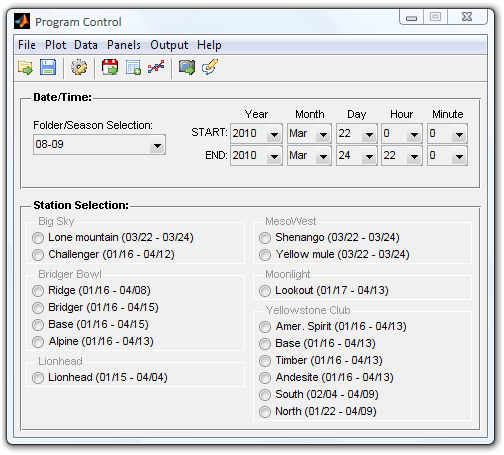
\includegraphics[width=4in]{\YCfiles figures/programcontrol.png}
	\caption{YCweather Program Control window.}\label{fig:programcontrol}
\end{figure}

\msusection{Tutorial: Plotting Weather Data}\label{sec:tutorial}
To quickly create a simple plot of weather data:
\begin{enumerate}
	\item Select a folder from the Folder/Season drop-down option on the Date/Time panel.
	\item Select a weather station from the buttons in the Station panel, for example Ridge and Bridger from Bridger Bowl.
	\item Choose a start and end date from the drop-down menus, be sure to select a range that lies within the available data, which is given in the parenthesis adjacent to the station radio buttons.	
	\item Select the Open Data List option.  This is available by selecting Open Data List option from the Data menu, pressing the Open Data List button on the toolbar, or by pressing CTRL + V.  This will open an additional window, as shown in Figure \ref{fig:datalist}. 
Note, this window may take several seconds to open especially if multiple stations are selected and/or if the stations contain a lot of data.  The reason being that when this window is open the program is recalling all of the data for each station and storing it in a temporary location. This allows the plots to be generated quickly.
	\item In this new window (named Data List) select a weather parameter, such as Air Temperature.  Notice, that when you press a button that all variables without the panel labeled Temperature disappear.  This will prevent plotting of variables with different units on the same axis.	
	\item Finally, plot the data.  This can be done by pressing the Plot Weather Data toolbar button on either Program Control or Data List window, by selecting Weather Data from the Plot menu on either window, and by CTRL + W.
\end{enumerate}

\begin{figure}[ht!]\centering
	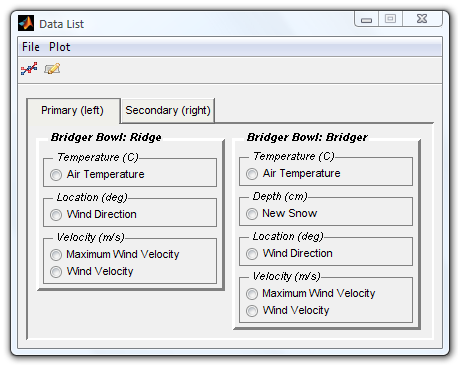
\includegraphics[width=4in]{\YCfiles figures/datalist.png}
	\caption{Example of the Data List window.}\label{fig:datalist}
\end{figure}

































\msusection{Creating Graphs}\label{YC:sec:graphs}
\newcommand{\nitem}[1]{\item{\textbf{#1}}}
One of the main purposes of YCweather is to produce graphs, these graphs are meant to be customizable and easily exportable.  This section details the creation and manipulation available in YCweather created graphs.  Graphs are generated using the Data List window as demonstrated in the previous section.

\msusubsection{Dual-axis}
When creating a graph, the Data List window (Figure \ref{fig:datalist}) displays two tabs.  Data selected via the Primary and Secondary tabs graph along the left-side and right-side vertical axis, respectively.  For example, Figure \ref{fig:dualaxis} was created by selecting Air Temperature under the Primary tab and Incoming Short-wave under the Secondary Tab. The tick marks along the axes are setup to coincide, this sometimes results in illogical tick mark labels.  This problem may be corrected by editing the limits and step size, which is detailed in the following section.

\begin{figure}[ht!]\centering
	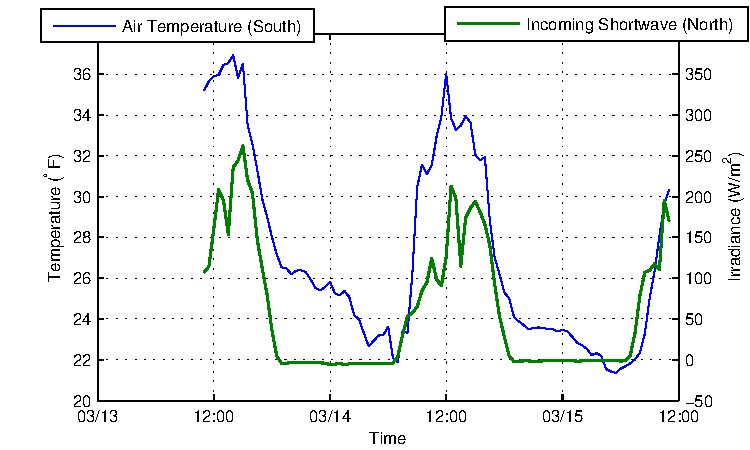
\includegraphics{\YCfiles figures/dualaxis.pdf}
	\caption{Example graph showing dual-axis capabilities.}
	\label{fig:dualaxis}
\end{figure}

\msusubsection{Editing Axis Limits and Step-size}\label{sec:editlimit}
In many cases, especially when creating graphs for dissemination, it is desirable to change the tick marks and limits on the graph.  YCweather provides this capability via two options: Limit Boxes and Step-size Boxes.  These options are available on the figure toolbar by the pairs of green arrows or by selecting the options from the corresponding axis menu (e.g., the X-axis menu).
\begin{itemize}
	\nitem{Limit Boxes:} This option creates two text box items near the extremes of the corresponding axis.  Simply change the limits to the desired value and press Enter.  If the box is empty the axis limits are automatically determined based on the data.
	\nitem{Step-size Boxes:} This toggle places a text box item near the lower axis limit.  This value dictates the step size between tick marks; leaving the value empty results in automatic tick placement.
\end{itemize}

\msusubsection{Exploring Data}\label{sec:exploredata}
The YCweather graphs allow the user to explore the data in various ways.

\begin{enumerate}
		\nitem{Limit/Step-size Boxes} allow for custom control of axis limits and tick marks, see Section \ref{sec:editlimit} for more details.
		\nitem{Zooming}: This option is toggled by selecting the magnifying glass icon on the figure toolbar. 
		\nitem{Data Cursor} allows the user to view the actual numbers associated with the graph by selecting a portion of the plotted line.  This option is available on the figure toolbar.
		\nitem{Zoom Slider} operates similar to the zooming feature but restricts the zoom to the associated axis and has a slider bar that controls the zooming from 100\% to 0.1\% of the data range.  The slider feature is available in the menus associated with each axis (e.g., X-Axis menu).
		\nitem{Line highlighting} is activated by left-clicking the mouse button on the desired line, this will make the line large and display the actual data points that make up the line.  The highlighting is removed by left-clicking the line a second time.
\end{enumerate}

\msusubsection{Context Menus}
The lines, labels, and legends on YCweather graphs each have menus associated that allow the user to manipulate the data.  The menus for these items are accessed by right-clicking on the object.

\begin{itemize}
	\nitem{Line Context Menu:}  By right clicking on any line the user has control over the appearance of the line for items such as the line thickness, style, color, or markers.  Additionally, a line may be deleted.
	\nitem{Label Context Menu:}  Each text item, such as the axis labels or annotations (see Section \ref{sec:axismenu}), allows for the user to edit the text, font, and location or delete the item. 
	\nitem{Legend Context Menu:}  The legend is also editable in its appearance including options for editing the color of the box or the width of the bounding box.  Also, when two legends are present. as in Figure \ref{fig:dualaxis}. they may be combined into a single legend by selecting the refresh option in this menu.  Then simply delete the unwanted legend box.
\end{itemize}
	
\msusubsection{Figure Menus}\label{sec:axismenu}
The axes menus available from graphs created with YCweather include the Options menu as well as a menu for each axis.  The Options menu provides generic functionality that applies to the entire figure whereas the axis specific menus only apply to that axis.

\msusubsubsection{File menu (default MATLAB menu)}
\begin{itemize}
	\nitem{New:} This option creates an empty figure, which is unaccessible with YCweather.
	\nitem{Open:} Allows the user to open figure files that were saved with the *.fig extension.
	\nitem{Close:} Closes the current figure.
	\nitem{Save:} Saves the figure by overwriting the current file if the figure has previously been saved, otherwise it envokes the Save as option.
	\nitem{Save as:} Allows the user to save the figure in a vareity of formats, including MATLAB *.fig format.
	\nitem{Export Setup:} Opens MATLAB's export user interface (see Section \ref{sec:exportfig}).
	\nitem{Print Preview:} Opens MATLAB's print setup user interface (see Section \ref{sec:exportfig}).
	\nitem{Print:} Sends the figure to the printer.
\end{itemize}

\msusubsubsection{Options menu}
\begin{itemize}
     \nitem{Add/Edit Labels:} Allows user to add and/or edit the axes labels, figure name, and figure title.
     \nitem{Interperter:} Allows user to change the typesetting format, \TeX\ and \LaTeX\ are usefull when equations and units are being displayed.
     \nitem{Edit Font:} Allows the user to change the font, style, and size for all text objects in the figure.
     \nitem{Axes Color:} Controls the background color of the figure.
     \nitem{Add Annotation:} Enables user to insert items such as text boxes and arrows.
     \nitem{Resize Figure:} Allows for editing the size of the figure, which is useful for exporting.
     \nitem{Tight Fit:} Moves the axis labels to the outer extent to minimize whitespace around the edges, this option is irreversible.
     \nitem{Export figure:} Allows the user to export the figure as an image file (see Section \ref{sec:exportfig}).
\end{itemize}

\msusubsubsection{X-,Y-, and Y2-Axis Menus}
\begin{itemize}
     \nitem{Ticks/Labels:} Allows for strict definition of the tick marks and labels used on the associated axis. 
     \nitem{Step Size Box:} Toggle for the step size controls (see Section \ref{sec:editlimit}).
     \nitem{Limit Boxes:} Toggle for the axis limit controls (see Section \ref{sec:editlimit}).
     \nitem{Zoom Slider:} Toggles the presence of the zoom slider (see Section \ref{sec:exploredata}).
     \nitem{Grid:} Toggles the major grid lines.
     \nitem{Minor Grid:} Toggles the minor grid lines.
     \nitem{Minor Ticks:} Toggles the axis tick marks.
     \nitem{Reversed:} Toggles the orientation of the tick marks and labels along the axis.
	 \nitem{Add/Edit Legend:} Allows the user to add or edit the legend entries.
\end{itemize}

\msusubsection{Exporting Figures}\label{sec:exportfig}
YCweather allows the user to output the graphs in a variety of formats.  For those familiar with MATLAB, it is possible save the figure as a *.fig file.  The exporting/saving is accomplished in two ways.  First, to simply create an image exactly as the figure appears, select Export Figure from the Options Menu or press the associated Toolbar button (see Section \ref{sec:axismenu}).  This option will output the figure exactly as it appears, so it is imperative to setup the figure precisely as needed.  The size of the exported figure can be specified by editing the dimensions via the Resize Figure option in the Options Menu.

The second option for saving/exporting figures is accomplished using the File Menu (Section \ref{sec:axismenu}), this menu is the default MATLAB figure menu; thus, for users unfamiliar with MATLAB these options may be difficult to use.  This menu provides two options: one for printing the image that uses the Print Preview and Print menu items and an Export Setup option for saving the figure as an image.  Both, the Print Preview and Export Setup open user interfaces with a variety of options, details for using these items may be found in the online MATLAB help file: \href{http://www.mathworks.com/access/helpdesk/help/techdoc/index.html}{\nolinkurl{http://www.mathworks.com/access/helpdesk/help/techdoc/index.html}} (in the contents select ``Graphics''; ``Printing and Exporting''; ``How to Print or Export'').


\msusection{Workspaces}\label{sec:workspace}
YCweather has the ability to save and load workspaces.  A workspace is simply a conglomeration windows including the Program Control, Data List, and any graphs.  For example, Figure \ref{fig:wsexample} is a workspace that includes graphs for air temperature and short-wave irradiance. 

\begin{figure}[h]\centering
	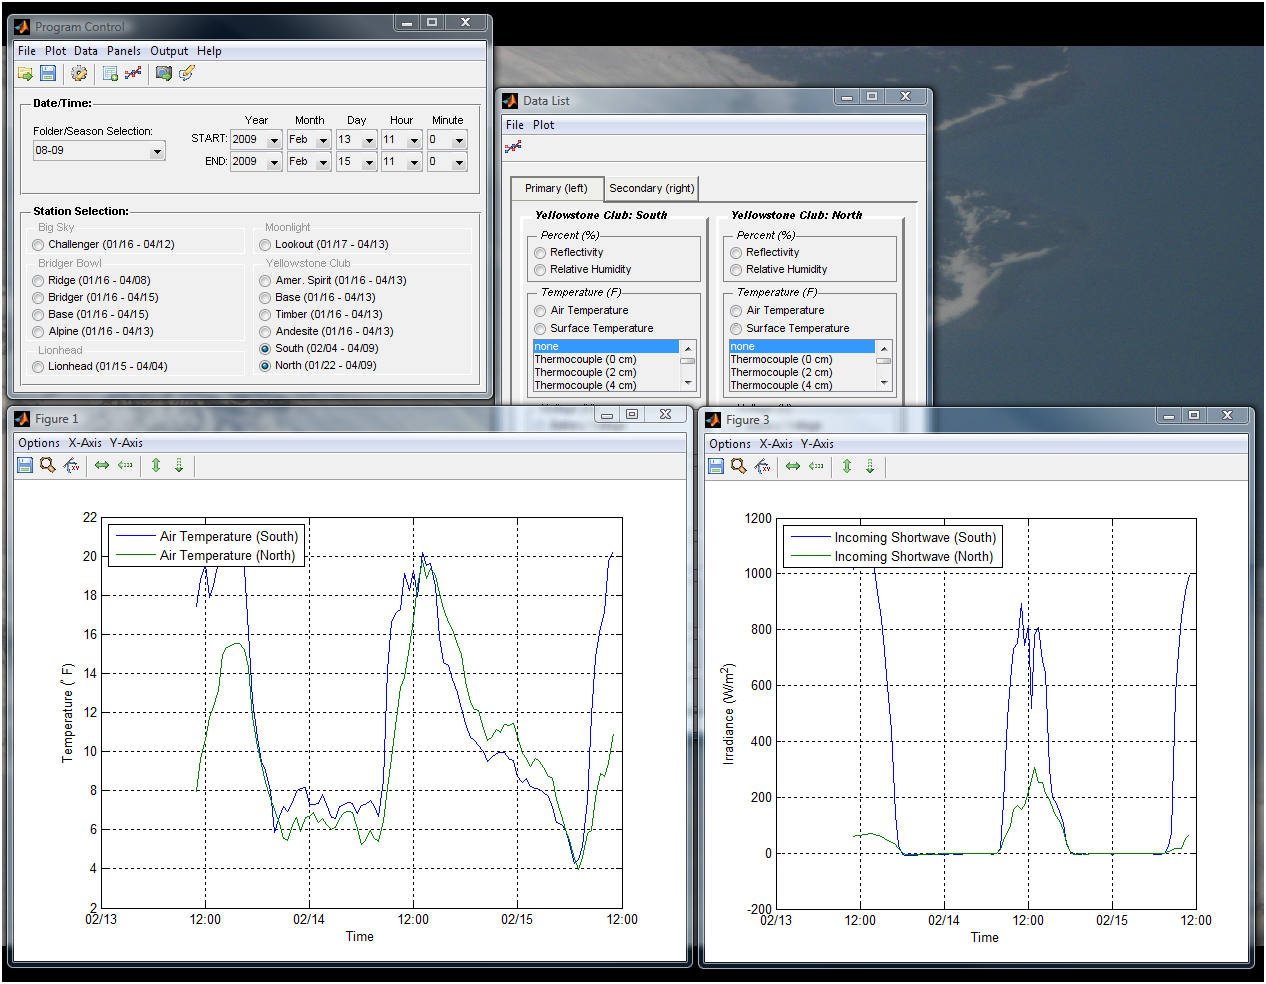
\includegraphics[width=\linewidth]{\YCfiles figures/wsexample.png}
	\caption{Example of a YCweather workspace.}
	\label{fig:wsexample}
\end{figure}

To create a workspace consider the following example:
\begin{enumerate}
	\item Begin by creating a graph of some kind, see Section \ref{sec:tutorial} for instruction on creating a graph.
	\item To create a second plot the Clear Figures preference must be turned off, see Section \ref{sec:pref} for details.
	\item Arrange the windows as desired.
	\item Save the workspace by selecting Save Workspace from the File menu in the Program Control window.  The default location is the \texttt{\bs saved} directory where YCweather was installed.  However, the workspace files (*.mat extension) may be saved in any location.
	\item The workspace is now saved.
\end{enumerate}

To load a workspace, simply select the Load Workspace option from the File menu and locate the desired workspace file in the dialog box that appears.  Once the workspace has been selected YCweather will provide a prompt, as in Figure \ref{fig:loadws}, that asks to use the current or stored time.  

\begin{figure}[ht!]\centering
	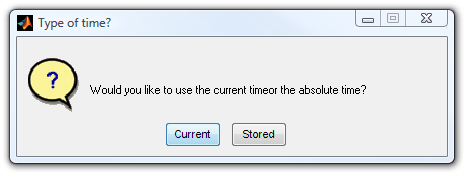
\includegraphics[width=0.55\linewidth]{\YCfiles figures/loadws.png}
	\caption{Prompt that appears by default when opening a workspace.}
	\label{fig:loadws}
\end{figure}

The ``current'' option, by default, recalls the workspace using the most recent 48 hrs of data that exists.  The stored time option uses the exact times set when the workspace was created.  These options exists so that the user can specify historical (``stored") workspaces of specific events or create workspaces (``current") of commonly used plots.  The YCweather preferences (Section \ref{sec:pref}) allow the number of hours to be changed as well as the prompt appearance to be changed.  For example, if a workspace is created that is solely intended for a specific event, then the prompting preference should be changed to ``Stored" so that when this workspace is recalled it simply opens.
\msusection{MesoWest Data}\label{sec:mesowest}
YCweather is capable of interfacing with weather data archived with MesoWest (\href{http://mesowest.utah.edu/index.html}{\nolinkurl{mesowest.utah.edu}}).  First, a text file names \texttt{mesowest.txt} must be present in the season folder within the YCweather database, see Section \ref{sec:database} for details regarding the folder structure.  This file contains three columns of comma separated data: the first column contains a list of station identifiers as shown on \href{http://mesowest.utah.edu/index.html}{MesoWest}.  For example, YLWM8 is the identifier for the Yellow Mule station in \href{http://mesowest.utah.edu/cgi-bin/droman/mesomap.cgi?state=MT&rawsflag=3}{Southwest Montana}.  The second column contains the desired name of the station (e.g., ``Yellow Mule'' for the above example). The third column contains a corresponding group name associated with the station identifier in the same row.  For example, the Yellow Mule station mentioned is a part of the RAWS network, thus an appropriate name may be ``RAWS Stations'' and perhaps another group would include the National Weather Service stations (e.g., ``NWS Stations'').

The data available for download from MesoWest is somewhat limited, as such the data is not actually downloaded until you select the station in the Program Control window. At this point YCweather will download the data based on the date range specified in the Program Control. Thus, if the data range is altered the station will be need to be reselected if the date range as been altered outside of the range previously selected. Also, the Data List will also need to be recreated. All of the MesoWest data may be updated via the Toolbar button or using the Data menu (see Section \ref{sec:data}).


\msusection{Preferences}\label{sec:pref}
YCweather offers a variety of customizable options for controlling how the program operates.  These options are available in the Preferences, which may be opened via the Program Control File menu or with the Toolbar button.  Figure \ref{fig:pref} shows the Preferences window.  This window is divided into three parts, each of which has a number of options as discussed below.

\begin{figure}[h]\centering
	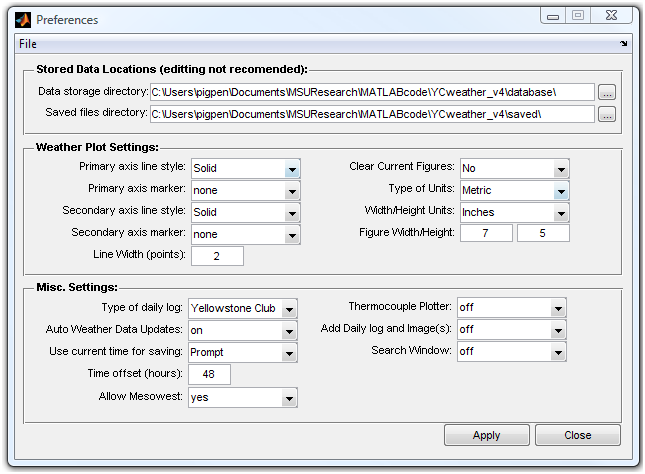
\includegraphics[width=\linewidth]{\YCfiles figures/pref.png}
	\caption{YCweather preferences window.}
	\label{fig:pref}
\end{figure}

In order for the changes in preferences to take place, the Apply button must be pressed.  The changed setting will only apply to the current YCweather workspace and will return to the default settings when YCweather is reopened.  The selected preferences may be defined as the default by selecting the Set Default option in the Preferences window File menu.  Additionally, if the workspace is saved (Section \ref{sec:workspace}) the current setting are applied to that workspace file and will remain when this workspace is opened in subsequent executions of this workspace file.

\msusubsection{Stored Data Locations}
As indicated in the Preferences window (Figure \ref{fig:pref}) editing the \q{database} and \q{saved} directory is not recommended unless a thorough understanding of file structure of YCweather is possessed.  These details are included in Section \ref{sec:advanced}, which discuss how YCweather operates. The \q{database} directory is where all the weather data, images, and log files are stored.  And the \q{saved} directory is the default location for all YCweather related files created by the user.

\msusubsection{Weather Plotting Settings}
The left-hand column in this section controls how the lines of weather graphs will appear upon creation, allowing for the adjustment of the line style, line markers, and line width for both the primary (left-side) and secondary (right-side) axes. The right-hand column includes various options, which are summarized in the following list.
\begin{itemize}
     \nitem{Clear Current Figures:} If this value is set to \q{Yes} then each time a graph is created all others are deleted.
     \nitem{Type of Units:} Specifies the units to display when graphs are created.  Note, if this is changed a new Data List window must be created because the unit conversion occurs during the creation of this window.
     \nitem{Width/Height Units:} Sets the units of the graph size upon creation, the numeric value for this setting is provided in the following item.
     \nitem{Figure Width/Height:} The width and height of a graph created based on the units specified above.
\end{itemize}

\msusubsection{Misc. Settings}
The settings in Misc. Settings panel, as the name suggests,  control various aspects of YCweather.  The first three items in the right-hand column toggle the appearance of the corresponding side panels when YCweather opens.  These panels are detailed in Section \ref{sec:panels}. 

The left-hand column allows the user to determine the type of daily log that YCweather should utilize, see Section \ref{sec:dailylogs} for details.  The Auto Weather Data Update options toggles the automatic download of the latest available weather data, as detailed in Section \ref{sec:data}.  The next  two options in this column control the graphing start and end times when graphs are created via workspaces, which is discussed in Section \ref{sec:workspace}. Finally, the ``Allow Mesowest'' setting toggles the capability for YCweather to communicate with the \href{http://mesowest.utah.edu/index.html}{MesoWest} database, which requires Internet access. Additional details regarding the \href{http://mesowest.utah.edu/index.html}{MesoWest} feature may be found in Section \ref{sec:mesowest}.

\msusection{Data Menu}\label{sec:data}
The Data menu in the Program Control window serves two functions: to access images and daily logs.

YCweather is relies on \href{https://dropbox.com}{Dropbox} to automatically collect the most recent weather data. For additional details please refer to the YCweather website: \link{aeslaughter.github.com/YCweather}.

\msusubsection{Image Viewer} \label{sec:images}
YCweather contains a basic image viewer for accessing images stored in the YCweather database.  Adding images to the database is explained in Section \ref{sec:add} and the database file structure is explained in Section \ref{sec:advanced}.  To access images, follow these steps:
\begin{enumerate}
	\item Select the station(s) of interest,
	\item Select the start date desired (the end date is not utilized), and
	\item Select Open Images from the Data menu or Toolbar button on the Program Control window.
\end{enumerate}

If images for the selected station(s) exist a window will open displaying the images. One window will appear for each station selected.  Figure \ref{fig:eximage} provides an example of the image window.  In the case where no images exist for selected date, but exist for other dates at this station, an image window will open with the Select Date pop-up menu (see Figure \ref{fig:eximage}) set to the first date available.  

\begin{figure}[ht!]\centering
	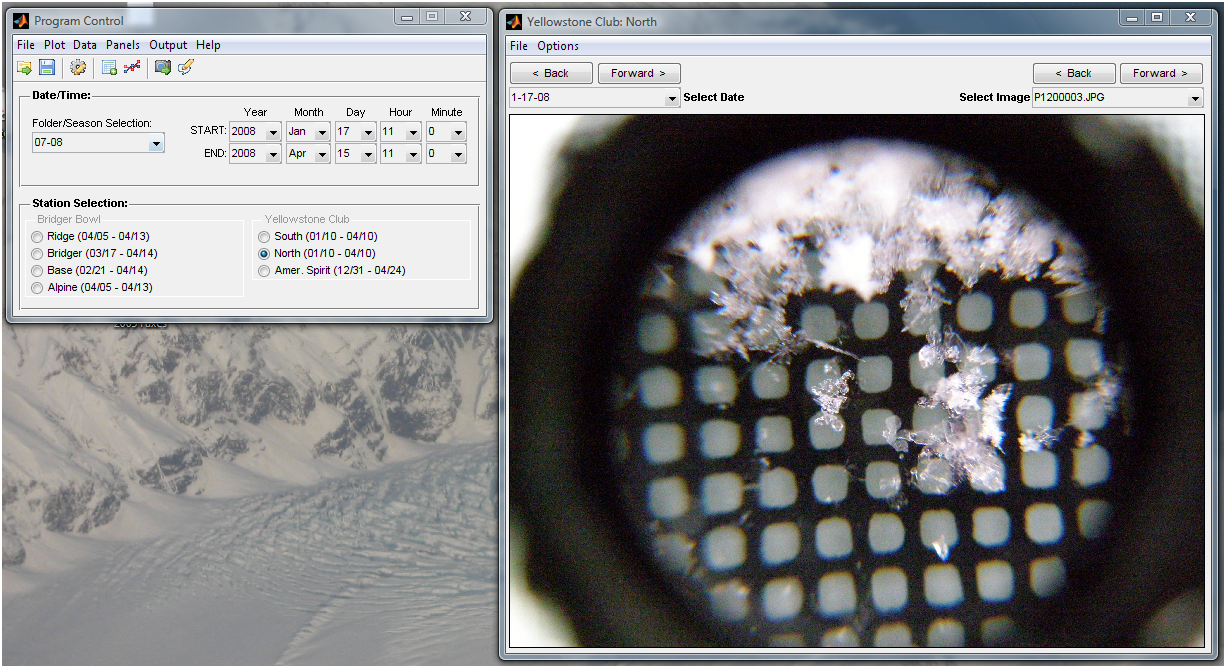
\includegraphics[width=\linewidth]{\YCfiles figures/eximage.png}
	\caption{Example of the image viewer for YCweather.}
	\label{fig:eximage}
\end{figure}

The YCweather image viewer offers the user the following functionality:
\begin{itemize}
     \item Toggles for cycling through images on the current date (right-hand buttons and pop-up menu).
     \item Toggles for changing the date being viewed (left-hand buttons and pop-up menu).
     \item Zooming via the mouse cursor.
     \item The ability to export the figure to another location via the Save image as\ldots ~option in the File menu of the image viewer (this copies the image and does not affect the original).
     \item Capability of renaming an image in the database (Rename in the Options menu).
     \item The ability of using the default Windows-based program for viewing images, which is available as the Open with Windows item in the Options menu. 
\end{itemize}

\msusubsection{Daily Logs} \label{sec:dailylogs}
One of YCweather's main features is the daily logs, which are text notes associated with each station and date.  These logs are stored in the YCweather database (see Section \ref{sec:advanced}) and added via the panel discussed in Section \ref{sec:add}.  Two types of daily logs are available, as shown in Figure \ref{fig:exlog}.  The type of log displayed is controlled in the preferences (Section \ref{sec:pref}).
\begin{enumerate}
	\nitem{Yellowstone Club: } A form specifically designed for usage with a research project at the Yellowstone Club.
	\nitem{General: } A simple form for typing notes.
\end{enumerate}

To open the daily logs: (1) select the station(s) of interest, (2) select the start date desired (the end date is not utilized), and
(3) chose Open Daily Log(s) from the Data menu or Toolbar on the Program Control window.

If daily logs exist then a window, similar to Figure \ref{fig:exlog}, will appear.  The toggles and pop-up menu on the right allow the user to cycle through all the logs for the station.   The daily log may be edited and the changes saved using the Save daily log option in the File menu. Additionally, the log may be opened in a traditional text editor (Open log with Windows in the Open menu); however, this is not recommended for the casual user. Editing the the log in this fashion may render the file unreadable by YCweather.  

It is possible to download images associated with the current station and date of the daily log, this is accessible by selecting Download images from the Open menu.  Finally, the image viewer for the current station may be opened using the daily log window by selecting Open images from the Open menu.

\begin{figure}[ht!]
	\subfloat[Yellowstone Club]{\label{fig:exlogYC}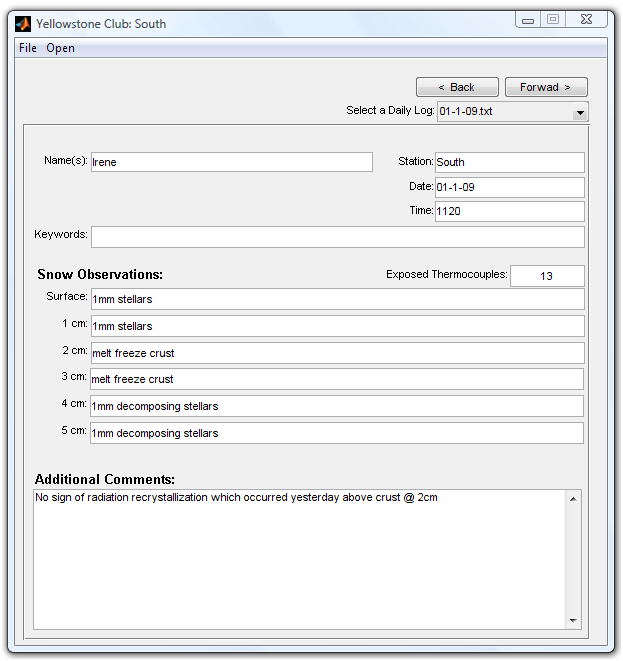
\includegraphics[width=0.49\linewidth]{\YCfiles figures/exlogYC.png}}\quad
	\subfloat[General]{\label{fig:exlogYC}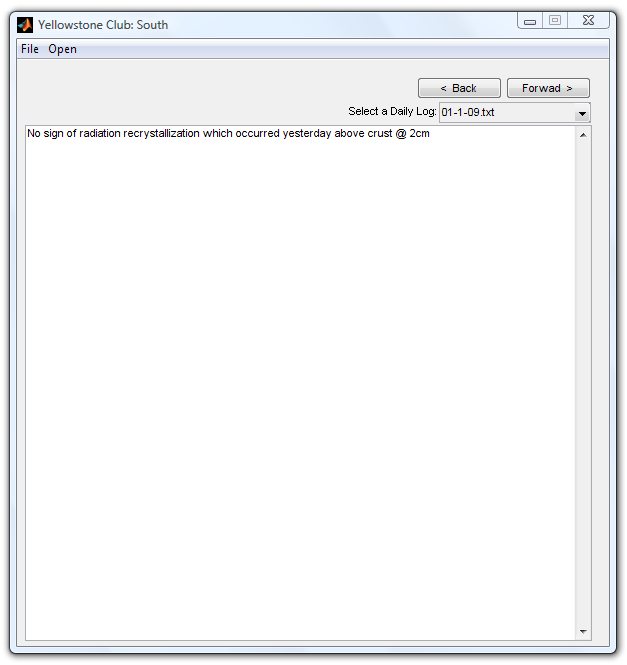
\includegraphics[width=0.49\linewidth]{\YCfiles figures/exlogGN.png}}
	\caption{Examples of the daily log options available in YCweather.}
	\label{fig:exlog}
\end{figure}

\msusection{Panels Menu}\label{sec:panels}
Three additional panels for manipulating data within YCweather are available: Thermocouple Plotter, Add Logs and Images, and Search.  These features are available via the Panels menu on the Program Control window.  These panels may be triggered automatically when YCweather opens via the program Preferences (Section \ref{sec:pref}).  Figure \ref{fig:panels} shows the Program Control window with all the panels.  Each of these panels servers a specific function, as defined below, that a typical user will likely not require.

\begin{figure}[h]\centering
	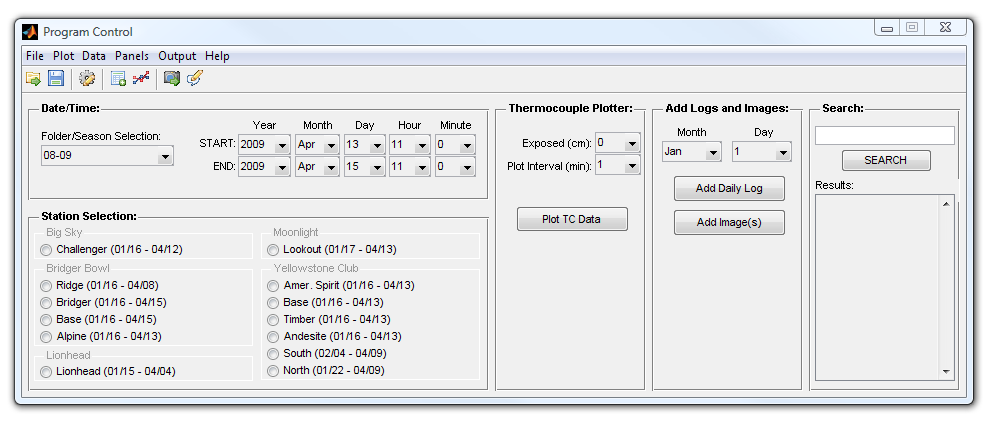
\includegraphics[width=\linewidth]{\YCfiles figures/panels.png}
	\caption{Program Control with all side panels showing.}
	\label{fig:panels}
\end{figure}

\msusubsection{Thermocouple Plotter}
A weather station may contain thermocouple data that extends into the snowpack, such as the North and South stations at the Yellowstone Club.  In this case it is desirable to graph temperature profiles of the snow pack at various intervals; the Thermocouple Plotter panel serves this purpose.  To understand this feature consider the following tutorial, referring to Figure \ref{fig:TCexample}.

\begin{enumerate}
	\item Open the Yellowstone Club South weather station Data List, as in Figure \ref{fig:TCexample}.  In the Data List window a list of thermocouple will be present in the Temperature panel, this indicates that this station has thermocouple data.
	\item Open the Thermocouple Plotter panel using the Panels menu on the Program Control window.
	\item Select a start and end time on the Program Control for just a few hours as in Figure \ref{fig:TCexample}.
	\item Change the Plot Interval pop-up menu to 30 minutes on the Thermocouple Plotter panel.
	\item Change the Exposed pop-up menu to a value of four.
	\item Press the Plot TC Data button.
\end{enumerate}

\begin{figure}[ht!]\centering
	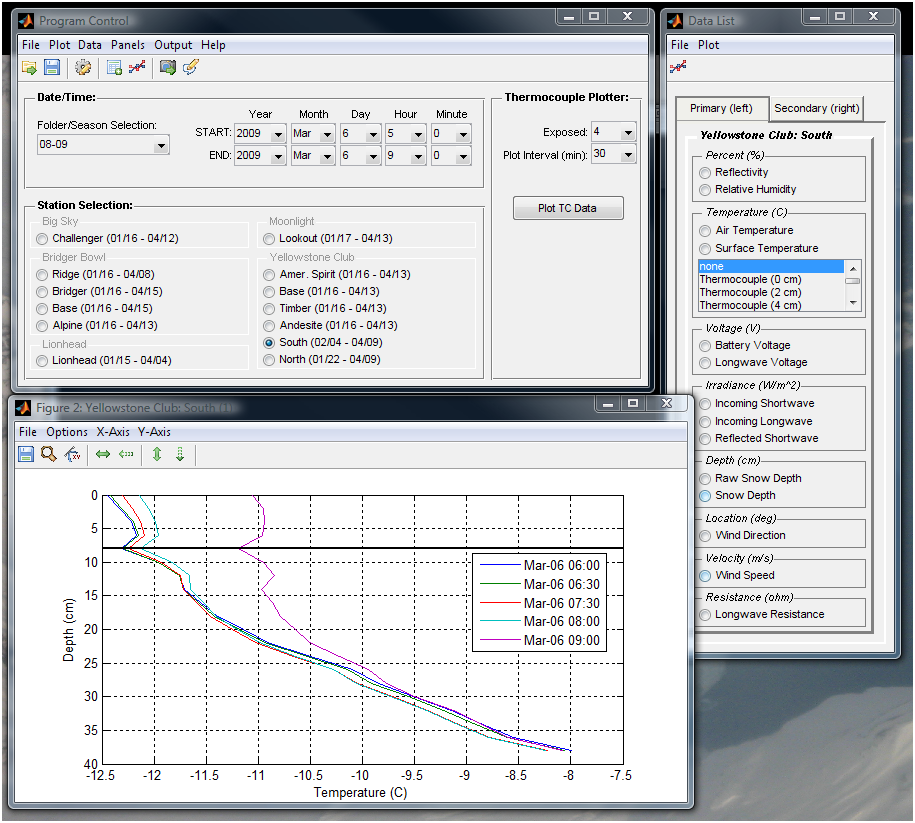
\includegraphics[width=\linewidth]{\YCfiles figures/TCexample.png}
	\caption{Example workspace showing a graph of thermocouple data.}
	\label{fig:TCexample}
\end{figure}

Following the above steps should produce a graph similar to that displayed in Figure \ref{fig:TCexample}.  This graph displays the theromocouple profiles at 30 minute intervals over the specified time.  The horizontal black line is meant to represent the snow surface.  For the North and South Yellowstone Club weather stations the number of thermocouples exposed is recorded in the daily logs.

\msusubsection{Add Logs and Images}\label{sec:add}
This panel allows the user to add image files and daily logs to a specific station for a specific date.  Each weather station (e.g. South at the Yellowstone Club or Ridge at Bridger Bowl) may have images and a daily log associated with the station for each day.  The Add Logs and Images panel allows this data to be assigned.  For example, to add a daily log for February 13 at the South Yellowstone Club station:
\begin{enumerate}
	\item select the South station from the Yellowstone Club panel in the Program Control window,
	\item select the appropriate day from the Add Logs and Images panel, and
	\item press the \q{Add Daily Log} button.
\end{enumerate}

Performing these steps opens a window for adding and editing the daily log.  Enter the desired information and then select the Save daily log option from the File menu.  If a log already exists for the selected station and date, a warning will appear.  If it is desired to overwrite the log then continue, otherwise the log should be edited.  Editing daily logs is discussed in \ref{sec:dailylogs}.

Similarly, images can be added to the YCweather database.  In this case the program will prompt the user to select the desired images to include, these images will be added to the database and accessible via the image viewer.  No changes to the images occur, YCweather simply builds a reference to the image file(s).  For specifics on the YCweather file organization within the database see Section \ref{sec:advanced}.

\msusubsection{Search}
The Search panel provides the user a tool for searching all the daily log (Section \ref{sec:dailylogs}) files for a specific folder/season.  Type the desired keyword(s) in the window with multiple words separated by a comma.  If any matches for any of the keywords exist the station and date will appear in the Results list.  Selecting the desired result opens the associated daily log.

\msusection{Output Menu}
\msusubsection{Output data to file(s)}
The weather data from YCweather may be exported as a comma separated text (*.txt), Microsoft Excel 97-2003 (*.xls), or Microsoft Excel 2007 (*.xlsx) file via the Output menu on the Program Control window. Selecting this option causes two options to appear:
\begin{itemize}
     \item \textbf{All data:} This option exports all the available weather variables, as listed in the Data list (Figure \ref{fig:datalist}),  from the selected stations.
	\item \textbf{Selected data:} This option only exports the data selected in the Data list (Figure \ref{fig:datalist}).
\end{itemize} 

After selecting one of these options YCweather will open a prompt asking: ``Would you like to crop the data between the selected date/times or write the entire data set?''  By selecting Crop only the data between the times selected on the Program Control window are exported. Selecting Entire exports all available data.

Next, YCweather will prompt for selecting the location and name of the output file, this is where the file type may be specified.  If either Excel file formats are selected YCweather will create a single file with each selected station as Worksheets within this file.  Outputting as a text file (*.txt) results in a file for each selected station being created, which will be named as \texttt{<name>\_station.txt}. The \texttt{<name>} is the filename entered by the user and the station is the YCweather designation for the station.

\msusubsection{Output to RadTherm}
YCweather is capable of producing a text file for the use with \href{HTTP://www.thermoanalytics.com/products/radthermrt/index.html}{RadTherm/RT} (ThermoAnalytics, Inc.), an example file is shown in Figure \ref{fig:radexport_a}.  This feature is accessed from the Output menu on the Program Control window.  This opens the RadTherm Export window, as shown in Figure \ref{fig:radexport_b}.

\begin{figure}[ht!]\centering
	\subfloat[]{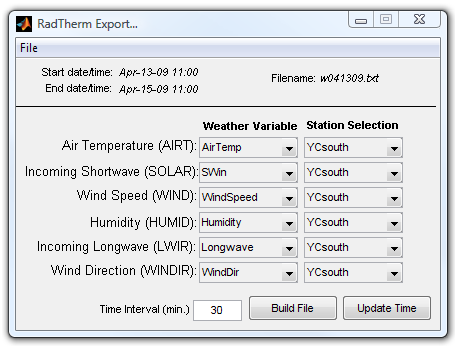
\includegraphics[width=0.48\linewidth]{\YCfiles figures/radexport_b.png}\label{fig:radexport_b}}\quad
	\subfloat[]{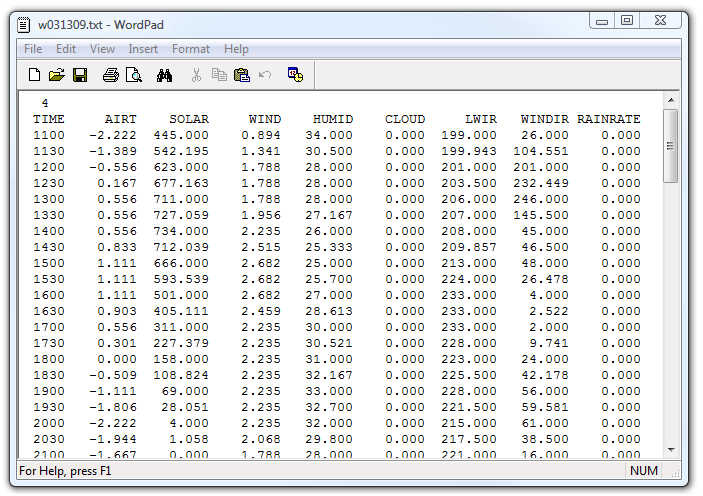
\includegraphics[width=0.48\linewidth]{\YCfiles figures/radexport_a.png}\label{fig:radexport_a}}
	\caption{(a) RadTherm/RT file exporter and (b) an example output file.}
	\label{fig:radexport}
\end{figure}

When using the exporter, begin by selecting the desired station from the right-column of pop-up menus.  When a station is selected the corresponding Weather Variable pop-up menu is changed to include weather variables with the necessary units.  The names that appear in both menus correspond to the tags assigned to the *.yc file for the stations, as discussed in Section \ref{sec:advanced}.  The start and end date/time values may be changed using the Program Control window and then by pressing the Update Time button.  Finally, the file is created by pressing Build File, a prompt will open for selecting the location to save the file.  The filename is dictated by the date.

The RadTherm/RT exporter also allows for the configuration of the pop-up menus to be saved.  This is available from the File menu on the exporter via the Save and Open Settings options.  These settings files utilize a *.rdt extension.

\msusection{Troubleshooting}
\msusubsection{Out-of-date MATLAB Compiler Runtime}
If after installing an update you receive the error shown in Figure \ref{fig:MCRerror} you must update the MATLAB Compiler Runtime. This is done by completing the following steps:
\begin{enumerate}
	\item Download and install \href{http://www.coe.montana.edu/ce/subzero/snow/}{MCRinstaller.exe} from the YCweather website. 
	\item Restart your computer.
	\item Reinstall YCweather, see Section \ref{sec:install}.
\end{enumerate}

\begin{figure}[H]\centering
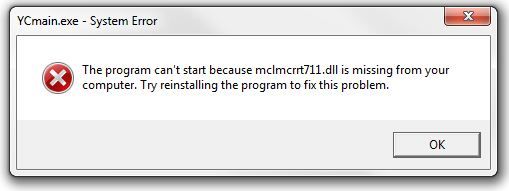
\includegraphics[width=0.66\linewidth]{figures/MCRerror.jpg}
\caption{Error message received when the MATLAB Compiler Runtime (MCR) requires updating.}
\label{fig:MCRerror}
\end{figure}

\msusection{Application Details} \label{sec:advanced}
The following section details of the operation of YCweather.  This section is meant to aid researchers at the Subzero Science and Engineering Research Facility maintain and update the software.  YCweather was written with MATLAB version 7.9.0.529 (R2009b).  If you are using a newer version of MATLAB for editting YCweather the MATLAB run time component must be updated on all machines attempting to execute YCweather (see Section \ref{sec:compile} for additional details).

\msusubsection{Source Code}
The source code for YCweather utilizes the \href{http://git-scm.com/}{git} version control system and the code may be pulled from \href{https://github.com/aeslaughter/YCweather}{github.com}. There a numerous Internet sources to aid in learning how to use both \href{http://git-scm.com/}{git} and \href{https://github.com/}{github}.

\msusubsection{Basic YCweather Operations}
The executable version of YCweather relies on four primary files that must be located in the same location: \texttt{YCweather.exe}, \texttt{YCmain.exe}, \texttt{default.mat}, and \texttt{version.txt}.  \texttt{YCweather.exe} is a wrapper program that keeps the main program \texttt{YCmain.exe} current based on the installed version (\texttt{version.txt}) and the available version on the YCweather website (Section \ref{sec:compile}).  \texttt{YCmain.exe} may be executed without \texttt{YCweather.exe}, but will never update in this case.  The source code for \texttt{YCweather.exe} and \texttt{YCmain.exe} are MATLAB m-files \texttt{YCweather.m} and \texttt{MAIN.m}, respectively.  \texttt{YCweather.m} will not operate correctly via the m-file; \texttt{MAIN.m} may be run via MATLAB if desired.

When \texttt{YCmain.exe} begins it opens the \texttt{default.mat} workspace file, which must be located in the same directory.  If this file does not exist or it is the first execution of YCweather this file is created.  The workspace file includes the location of the database directory that contains all the weather data, daily logs, and image files.  This directory may be located anywhere on the machine as long as the workspace file points to the correct location (see Sections \ref{sec:pref}).  However, when the \texttt{default.mat} workspace file is created the location is initially set as the \q{database} folder in the same directory as the YCweather executables.

When \texttt{YCmain.exe} (\texttt{MAIN.m}) begins operation, after opening the workspace file (\texttt{default.mat}), it attempts to download the latest weather data.  As mentioned in Section \ref{sec:data} this option may be turned off.  The installation package, Section \ref{sec:compile}, includes the latest data from the current season.  Thus, an Internet connection is not required to run YCweather initially, but only to keep the program and data current.  Lastly, \texttt{YCmain.m} initializes by applying the \texttt{default.mat} workspace file (\texttt{callback\_readWS.m}), prior to this the only two parameters in the workspace file where utilized: the database location and the auto update trigger.

At this point, the YCweather is ready for manipulation by the user and the program has opened all available data into the internal data structures.

\msusubsection{Database Directory}\label{sec:database}
The database directory must be organized in a specific fashion for YCweather to operate correctly, most of this organization is handled automatically.  The directory tree for the YCweather database is shown in Figure \ref{fig:filestructure}.  The first level of folders in the database directory are for each season of data, these exact folder names show up in the Program Control window in the Season/Folder pop-up menu.  The initialization of the pop-up menu occurs when a workspace file is opened, the source code being \texttt{callback\_readWS.m}.

When the user selects the season via the pop-up menu YCweather accesses this folder, inside of which the *.yc format files (see Section \ref{sec:formatfile}) for all weather stations are stored.  These format files contain, among other things, an abbreviated station name.  This name is used in the internal data structure of YCweather as well as for creating the next level of folders.

As described in Section \ref{sec:data}, YCweather acts as an archiving application for daily logs and images.  The daily logs, images, or image reference files are contained in folders that exist within the station folders.  The folders are named according the aforementioned abbreviated station name.  Within each of these folders two additional folders exist: DailyLogs and Images.  These folders, as the names suggest, store the archived daily logs and image files.  The station folders and sub-folders are created automatically by YCweather when the user adds a daily log or image (see Section \ref{sec:add}).

The DailyLog folder contains text files that store the daily log information, each log must me named as \texttt{mm-dd-yy.txt}.  The Images folder contains folders named as \texttt{mm-dd-yy}.  Within each folder the images are stored, the names are irrelevant, but the files should be stored only in recognized formats, see MATLAB's help on \q{imread}.  This directory may also contain a \texttt{images.txt} file which contains a list of image files elsewhere on the computer that have been associated with the station and data by the user, see Section \ref{sec:add}.

\begin{figure}[h]\centering
	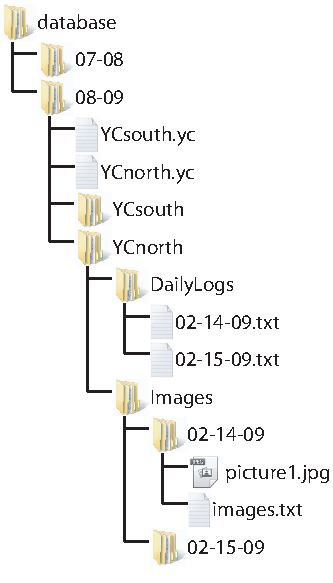
\includegraphics[]{\YCfiles figures/filestructure.pdf}
	\caption{Example of file structure of the database directory used by YCweather.}
	\label{fig:filestructure}
\end{figure}

\msusubsection{Weather Station Format Files (*.yc)}\label{sec:formatfile}
YCweather basis it's entire operation on format files, which are simply text files with a *.yc extension.  An example, format file is include in Figure \ref{fig:formatfile}.  These files communicate to YCweather the necessary information regarding the weather data files.  The weather data files may be any comma delimited text file completely composed of columnar numeric entries.

\begin{figure}[h]\centering
	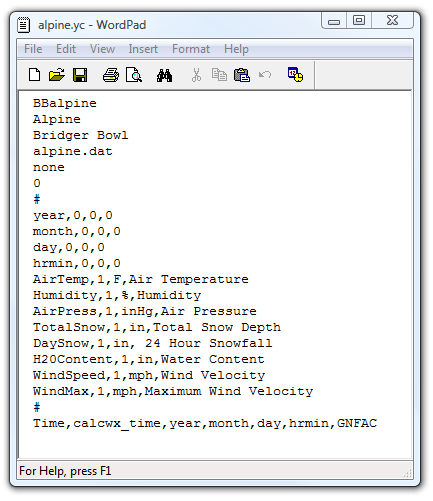
\includegraphics[width=0.55\linewidth]{\YCfiles figures/formatfile}
	\caption{Example format file utilzed by YCweather.}
	\label{fig:formatfile}
\end{figure}

Format files are composed of three parts, with the parts being separated by \# sign.  The first portion consists of six lines that detail various parts of the data file.  Part two details each column of data present in the data file.  Finally, part three contains custom functions utilized for making calculations.

\msusubsubsection{Part One: Data File Details}
The following list is a line-by-line description of the six components required in the first portion of the *.yc format files.

\begin{enumerate}
	\nitem{Station ID:} The station id must be a single text string that uniquely identifies the weather station associated with this data file.  This ID must conform to MATLAB's variable naming convention, see MATLAB's help file on \q{Naming Variables}.
	\nitem{Station name:} This string identifies the weather station and will appear next to the toggle button within the Station Panel in the Program Control window.
	\nitem{Station location:} This value is a text string that identifies the location of the weather station, this name will appear in the Station Panel in the Program Control Window.
	\nitem{Path to data file:} The path to the data file must be any valid complete or relative path and filename that references the data file associated with this format file.  In the example file, Figure \ref{fig:formatfile}, the file \texttt{alpine.dat} must then exist in the same directory as the *.yc format file.
	\nitem{Array ID:} This value is useful for weather files that are composed of multiple data arrays such as created via Campbell Scientific dataloggers.  In many cases data files of this type contain a identifier at the beginning of a row identify the type of data.  For example, a row beginning with 60 may represent hourly data and those starting with 24 may indicate daily data.  Thus, if the Array ID is 60 in the *.yc format file then only the data marked with this ID would be included for this station in YCweather.  Another *.yc file would need to be established to gather the data from the other array.  Figure \ref{fig:formatfile2} includes the Array ID feature.  In Array ID is present in the file, \texttt{none} should be entered in this location.
	\nitem{Thermocouple ID:} This identifier indicates if a thermocouple array within the snowpack exists.  If this data does not exist then \texttt{0} (zero) should be entered.  For stations with snowpack temperature arrays this ID should correspond the the variable ID's defined in part two of the *.yc file, as discussed below and shown in Figure \ref{fig:formatfile2}.  The variable ID also must contain a numeric portion that indicates the location of each thermocouple in the snowpack.  For example, the thermocouples shown in Figure \ref{fig:formatfile2} are space at 2 cm intervals.
\end{enumerate}

\begin{figure}[!ht]\centering
	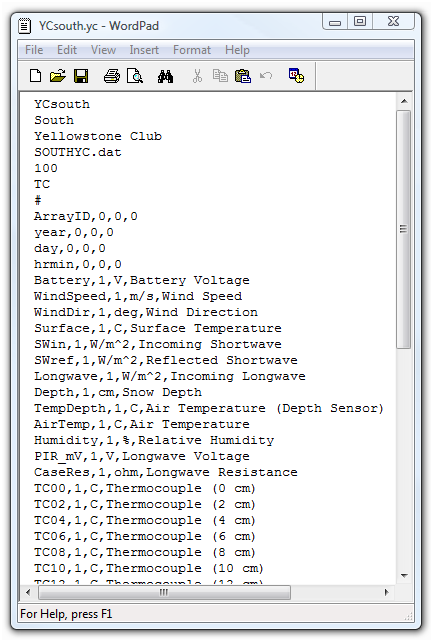
\includegraphics[width=0.55\linewidth]{\YCfiles figures/formatfile2}
	\caption{Example format file utilized by YCweather that includes the thermocouple ID for plotting temperature profile data (this is not a complete file).}
	\label{fig:formatfile2}
\end{figure}

\msusubsubsection{Part Two: Weather Variables}
Part two details the weather variables, there should be one row for each column that exists in the corresponding data file.  Each row in this section has four comma separated values, as detailed below.

\begin{enumerate}
	\nitem{Variable Name:} The first value is a single string of text that uniquely defines the variable from others in the format file. This name must conform to MATLAB's variable naming convention, see MATLAB's help file on \q{Naming Variables}.
	\nitem{Inclusion Trigger:} This value indicates to YCweather if the corresponding column of data should be listed as a selectable option in the program.  Entries may be 0 or 1, where 0 excludes the data.
	\nitem{Units:} The third entry communicates the units of the data; this value must conform to the units specified in the \texttt{units.txt} file as detailed in Section \ref{sec:units}.  The units can be in either English or metric units, but must be included in the aforementioned file.
	\nitem{Legend Label:} The last value is a string describing the weather data that is inserted into the legends of YCweather graphs.
\end{enumerate}

\msusubsubsection{Part Three: Custom Functions}
This section allows for calculation to be done on the weather variables listed above in Part Two.  One function that is a critical component of YCweather will be used here as an example, the \texttt{calcwx\_time.m} function. \textbf{YCweather requires that a variable named \texttt{Time} be present and contain the time stamps for the weather data in MATLAB's serial format.} The \texttt{calcwx\_time.m} function performs this operation. For information on this format see MATLAB's help on \q{Types of Date Formats}.  

Taking a step back, the function \texttt{read\_dat.m} is responsible for reading the format *.yc files, this function outputs the weather data into a structure that is used by YCweather; \texttt{read\_dat.m} also implements the custom functions listed in the *.yc format files.

When the custom function are called from \texttt{read\_dat.m} they are implemented as follows within MATLAB, using \texttt{calcwx\_time.m} as an example.
\begin{Verbatim}[fontsize=\small , frame=single, label=MATLAB]
>> Time = calcwx_time(d,'year','month','day','hrmin','GNFAC');
\end{Verbatim}

Comparing this functional operation to the row of inputs in the format file in Figure \ref{fig:formatfile} shows that the first entry in the format *.yc file is the output variable (\texttt{Time}), the next value is the function name (\texttt{calcwx\_time}), and the remaining items are string input into the custom function.  The input variable d is the data structure used for storing the weather data and is automatically inputed into the custom function in \texttt{read\_dat.m}.  This data structure contains all the data present in the weather data file, as listed in Part Two.  Hence, the function \texttt{calcwx\_time.m} uses the input strings (\texttt{'year','month'}, etc.) to compute the new Time variable with the appropriate time format required by YCweather.  So, each custom function essentially creates another weather variable for use by YCweather.

The custom functions were setup to allow YCweather to be expandable by the user to perform calculations on the weather data.  To best understand the custom functions, it is best to examine the source code, specifically section five of \texttt{read\_dat.m} and any of the existing custom functions: \texttt{calcwx\_time.m, calcwx\_flux.m}, and \texttt{calcwx\_labLW.m}.

\msusubsection{Variable Units}\label{sec:units}
As mentioned in Section \ref{sec:formatfile}, the format files require that the units for each weather variable be defined.  The units prescribed in the format file must be present in the \texttt{units.txt} file, which is read by the \texttt{getunit.m} function.  The \texttt{units.txt} defines the units via text abbreviations (e.g., \texttt{'kPa'} for pressure) both in Metric and English, the conversion factor between the units, and the appropriate axis labels for use in YCweather generated graphs. The function \texttt{getunit.m} is utilized for extracting the various unit related information in various portions of YCweather.  Both the function \texttt{getunit.m} and text file \texttt{units.txt} were designed to allow for additional units to be added, which should only require adding a row to the text file. 

The \texttt{units.txt} file should be composed of rows containing the following comma separated information: 1) the Metric abbreviation, 2) the English abbreviation, 3) text describing the unit, 4) the Metric abbreviation written in \LaTeX ~math format, 5) the English abbreviation written in \LaTeX ~math format, 6) the Metric unit written as \TeX, 7) the English unit written as \TeX, 7), and finally 8) the conversion multiplier from English to Metric.  Figure \ref{fig:units} contains a portion of the \texttt{units.txt} file, refer to the file itself for additional examples as well as additional information regarding the format.  Note, the \# is the comment character within the file.

\begin{figure}[!ht]\centering
	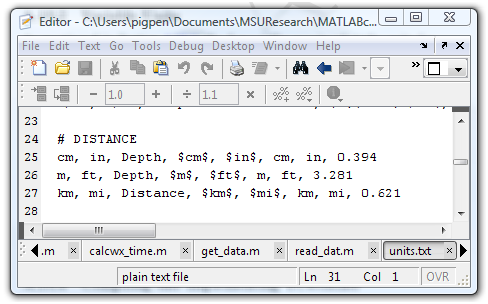
\includegraphics[width=0.55\linewidth]{\YCfiles figures/units.png}
	\caption{Example entries for prescribing units within the \texttt{units.txt} file, which is utilized by the \texttt{getunit.m} function.}
	\label{fig:units}
\end{figure}

\msusubsection{Compiling and Implementing YCweather}\label{sec:compile}
The information in this section details the process for building a YCweather executable file from the source code via MATLAB's compiler. Note, that if a 32-bit version of MATLAB is being used the compiler is included, otherwise a compiler must be installed (see \href{http://www.mathworks.com/support/compilers/R2010a/}{\nolinkurl{www.mathworks.com/support/compilers/R2010a/}}). The \texttt{mbuild -setup} function in MATLAB is used to setup your compiler initially.  

If any changes are made to the source code of YCweather the following information will make the updates available to all users running YCweather. The function \texttt{YCbuild.m} acts to automate the process of compiling YCweather into executable form as well as post the updated to the web folder.  The function requires two outside programs, WinSCP\footnote{\href{http://winscp.net}{WinSCP: winscp.net}} and InstallJammer\footnote{\href{http://www.installjammer.com/}{InstallJammer: www.installjammer.com}}.

After changing the source code, implement the the following code from the MATLAB command-line: \texttt{>>YCbuild('build',0.5)}, where the second input is the new version number.  When this command executes the version is updated, YCweather.exe and YCmean.exe are complied, YCmain.zip is packaged, the latest weather data from the current season is prepared, and the installer is compiled (YCinstaller.exe).  All of these files are placed in the \texttt{release} directory, which are exactly the files need on the YCweather website.  Before compiling a new version, the version number in the \texttt{MAIN.m} functions should be updated.

This process relies on three files.  First, the two project files: YCweather.prj and YCmain.prj.  These files were created with MATLAB's \texttt{deploytool} and dictate how YCweather.exe and YCmain.exe are compilied.  If any additional m-files are added to YCweather then these files will needed to be added to the list of files in the YCmain.prj file.  The third file, is the InstallJammer installation file, YCinstaller.mpi, which is stored in the YCinstallerFiles directory.

Once YCweather is complied it must also be uploaded to the website so that the changes will be made available to all users of the program.  This is done by executing the following: \texttt{>>YCbuild('web')}.  This removes the old files from the web and adds the new via WinSCP; access to the appropriate account on the MSU Department of Civil Engineering server is required. 

\msusubsection{Website and Online Weather Database}\label{sec:web}
The YCweather website, \href{http://www.coe.montana.edu/ce/subzero/snow/}{www.coe.montana.edu/ce/subzero/snow}, is hosted by the MSU College of Engineering and contains the installation files YCweather and the files for automatically updating YCweather.  These files are automatically generated during the compilation and posting process described in Section \ref{sec:compile}.

YCweather also relies on an ftp accessible database hosted by the College of Engineering, which contains the weather files database directories that are accessed by YCweather for keeping the weather data up to date.  The MATLAB program \texttt{GNAFC.m} located on the server is executed hourly to keep the weather data current via CRONTAB.

%\msusection{MATLAB Source Code}
The following list includes all the files associated with YCweather and a short description of the program.\par
\newcommand{\MATLABitem}[2]{\item \hyperref[mfile:#1]{\bfseries #2}: \label{mlist:#1}}
\newcommand{\MATLABsubitem}[1]{\item{\bfseries #1}: }
\begin{itemize}[itemsep=0pt]
    \MATLABitem{DailylogGUI}{DailylogGUI.m} M-file for DailylogGUI.fig
    \MATLABitem{ImageGUI}{ImageGUI.m} M-file for ImageGUI.fig
    \MATLABitem{MAIN}{MAIN.m} is the controlling program for the YCweather software.
    \MATLABitem{Plotmenus}{Plotmenus.m} builds the variable list for each station listed in "sta" and
    \MATLABitem{WorkspaceGUI}{WorkspaceGUI.m} M-file for WorkspaceGUI.fig generated using MATLAB's Guide
    \MATLABitem{XYscatter}{XYscatter.m} is custom plotting program based on MATLAB plot function.
    \MATLABitem{YCbuild}{YCbuild.m} compiles and posts the YCweather software package
    \MATLABitem{YCweather}{YCweather.m} is the front end to YCmain.exe program.
    \MATLABitem{applysettings}{applysettings.m} captures, inserts, or apply the program settings based on
    \MATLABitem{buildsidebars}{buildsidebars.m} constructs panels that attach to the side of the main
    \MATLABitem{calcwxflux}{calcwx\_flux.m} calculates the fluxes and related properties for YCweather
    \MATLABitem{calcwxlabLW}{calcwx\_labLW.m} 
    \MATLABitem{calcwxtime}{calcwx\_time.m} converts time data into MATLAB serial format
    \MATLABitem{callbackadd}{callback\_add.m} log enables user to add a new daily log to database
    \MATLABitem{callbackclick}{callback\_click.m} operates when the user selects a variable.
    \MATLABitem{callbackexport}{callback\_export.m} allows user to export data to *.txt or *.xlsx files
    \MATLABitem{callbackexportTHERMAL}{callback\_exportTHERMAL.m} opens a GUI for exporting data to thermal model
    \MATLABitem{callbackopenimage}{callback\_openimage.m} opens an image viewer for each station selected;
    \MATLABitem{callbackopenlog}{callback\_openlog.m} 
    \MATLABitem{callbackplotTCdata}{callback\_plotTCdata.m} plots thermocouple data with depth
    \MATLABitem{callbackplotdata}{callback\_plotdata.m} plots the selected data.
    \MATLABitem{callbackpref}{callback\_pref.m} 
    \MATLABitem{callbackpress}{callback\_press.m} operates when the secondary or primary button is pressed
    \MATLABitem{callbackreadWS}{callback\_readWS.m} 
    \MATLABitem{callbackrecent}{callback\_recent.m} builds and maintains the open recent list in file menu
    \MATLABitem{callbacksaveWS}{callback\_saveWS.m} - saves tge current workspace to a *.mat file
    \MATLABitem{callbacksearch}{callback\_search.m} uses the keywords entered in the daily logs text files
    \MATLABitem{callbackseason}{callback\_season.m} updates the data displayed by YCweather
    \MATLABitem{callbacksettime}{callback\_settime.m} executes when user changes the start/end times
    \MATLABitem{callbacksidebar}{callback\_sidebar.m} opens or closes sidebars (i.e. items from the Window
    \MATLABitem{callbackvarmenu}{callback\_varmenu.m} is the callback function for the MAIN program that opens
    \MATLABitem{errorlog}{errorlog.m} saves error information to errorlog.txt
    \MATLABitem{getdata}{get\_data.m} extracts the data from the a variable
    \MATLABitem{getselected}{getselected.m} builds a cell array of the selected stations.
    \MATLABitem{getunit}{getunit.m} returns unit information or converts units.
    \MATLABitem{groupitems}{group\_items.m} 
    \MATLABitem{logviewer}{log\_viewer.m} opens a GUI to view images.
    \MATLABitem{prefGUI}{prefGUI.m} M-file for prefGUI.fig as created using GUIDE
    \MATLABitem{radthermGUI}{radthermGUI.m} M-file for radthermGUI.fig
    \MATLABitem{readdat}{read\_dat.m} reads data from the station *.yc format file and builds a data
    \MATLABitem{syncdata}{syncdata.m} sychronizes database with current weather data
    \MATLABitem{thermGUI}{thermGUI.m} M-file for thermGUI.fig
    \MATLABitem{waitbar}{waitbar.m} a modified version of MATLAB's waitbar function.
\end{itemize}

\newcommand{\codedir}{C:/Users/pigpen/Documents/MSUResearch/MATLABcode/YCweather_v4/}
\newcommand{\verbcode}[3]
{
\subsection{\bfseries \hyperref[mlist:#1]{#2} Program Code \label{mfile:#1}}
\VerbatimInput[frame=single,framesep=2mm,label=#2,numbers=left,numbersep=2pt,fontfamily=tt,fontsize=\footnotesize]{\codedir #3}
}
\verbcode{DailylogGUI}{DailylogGUI.m}{DailylogGUI.m}
\verbcode{ImageGUI}{ImageGUI.m}{ImageGUI.m}
\verbcode{MAIN}{MAIN.m}{MAIN.m}
\verbcode{Plotmenus}{Plotmenus.m}{Plotmenus.m}
\verbcode{WorkspaceGUI}{WorkspaceGUI.m}{WorkspaceGUI.m}
\verbcode{XYscatter}{XYscatter.m}{XYscatter.m}
\verbcode{YCbuild}{YCbuild.m}{YCbuild.m}
\verbcode{YCweather}{YCweather.m}{YCweather.m}
\verbcode{applysettings}{applysettings.m}{applysettings.m}
\verbcode{buildsidebars}{buildsidebars.m}{buildsidebars.m}
\verbcode{calcwxflux}{calcwx\_flux.m}{calcwx_flux.m}
\verbcode{calcwxlabLW}{calcwx\_labLW.m}{calcwx_labLW.m}
\verbcode{calcwxtime}{calcwx\_time.m}{calcwx_time.m}
\verbcode{callbackadd}{callback\_add.m}{callback_add.m}
\verbcode{callbackclick}{callback\_click.m}{callback_click.m}
\verbcode{callbackexport}{callback\_export.m}{callback_export.m}
\verbcode{callbackexportTHERMAL}{callback\_exportTHERMAL.m}{callback_exportTHERMAL.m}
\verbcode{callbackopenimage}{callback\_openimage.m}{callback_openimage.m}
\verbcode{callbackopenlog}{callback\_openlog.m}{callback_openlog.m}
\verbcode{callbackplotTCdata}{callback\_plotTCdata.m}{callback_plotTCdata.m}
\verbcode{callbackplotdata}{callback\_plotdata.m}{callback_plotdata.m}
\verbcode{callbackpref}{callback\_pref.m}{callback_pref.m}
\verbcode{callbackpress}{callback\_press.m}{callback_press.m}
\verbcode{callbackreadWS}{callback\_readWS.m}{callback_readWS.m}
\verbcode{callbackrecent}{callback\_recent.m}{callback_recent.m}
\verbcode{callbacksaveWS}{callback\_saveWS.m}{callback_saveWS.m}
\verbcode{callbacksearch}{callback\_search.m}{callback_search.m}
\verbcode{callbackseason}{callback\_season.m}{callback_season.m}
\verbcode{callbacksettime}{callback\_settime.m}{callback_settime.m}
\verbcode{callbacksidebar}{callback\_sidebar.m}{callback_sidebar.m}
\verbcode{callbackvarmenu}{callback\_varmenu.m}{callback_varmenu.m}
\verbcode{errorlog}{errorlog.m}{errorlog.m}
\verbcode{getdata}{get\_data.m}{get_data.m}
\verbcode{getselected}{getselected.m}{getselected.m}
\verbcode{getunit}{getunit.m}{getunit.m}
\verbcode{groupitems}{group\_items.m}{group_items.m}
\verbcode{logviewer}{log\_viewer.m}{log_viewer.m}
\verbcode{prefGUI}{prefGUI.m}{prefGUI.m}
\verbcode{radthermGUI}{radthermGUI.m}{radthermGUI.m}
\verbcode{readdat}{read\_dat.m}{read_dat.m}
\verbcode{syncdata}{syncdata.m}{syncdata.m}
\verbcode{thermGUI}{thermGUI.m}{thermGUI.m}
\verbcode{waitbar}{waitbar.m}{waitbar.m}


% == SECTION: Bibliography ==========================================
% \clearpage\newpage
% \addtocounter{section}{1}
% \addcontentsline{toc}{section}{Bibliography} 
% \renewcommand\refname{\thesection Bibliography}
% \bibliographystyle{ametsoc}
% \bibliography{research}{}
\end{document}